% Chapter Template

\chapter{CARACTERIZACION DE UN BMG BAJO DIFERENTES MODOS DE CARGA Y TEMPERATURAS} % Main chapter title

\label{C3} % Change X to a consecutive number; for referencing this chapter elsewhere, use \ref{ChapterX}

\lhead{Capítulo 3. \emph{CARACTERIZACION DE UN BMG}} % Change X to a consecutive number; this is for the header on each page - perhaps a shortened title

%----------------------------------------------------------------------------------------
%	SECTION 1
%----------------------------------------------------------------------------------------
%\section{Abstract}

%Amorphous metals, i.e. without defined crystal structure; are increasingly used in modern life, showing great potential as advanced engineering materials, due to some of its characteristic properties such as high hardness and moldability, high resilience, high mechanical strength and high wear resistance, among others. All these properties allow obtaining parts with complex shapes and high strength, which increases their chances for industrial application. However, many details of the mechanical behavior are still unknown, and the currently used models and theories are far from predictive.
%One of the possibilities to determine constitutive parameters, and thus study the response of these materials, is by using atomistic calculations. In this paper we present results obtained with molecular dynamics (MD) simulations, of an amorphous metal (CuZr). In particular, constitutive parameters such as elasticity modulus, are determined for samples at different temperatures and subjected to both tension and compression. The results obtained are relevant for understanding the mechanical behavior of the material, such as stress-strain and temperature-strain relationships. Additionally, it is possible to observe, under uniaxial tension, the nucleation and growth of a void due to high stress and strain rate values.

\section{Introducción}
\label{S3_1}

%Los materiales sólidos sin una estructura ordenada, es decir, amorfos, son llamados generalmente "vidrios". Algunos casos particulares de gran interés científico y tecnológico son los vidrios metálicos, que son aleaciones metálicas con propiedades mecánicas que sobrepasan en prestaciones a las aleaciones cristalinas más comunes (\cite{luborsky83}, \cite{greer95}). Se sabe que los metales forman fácilmente cristales cuando son enfriados (\cite{callister95}, \cite{smith96}). Sin embargo, usando una velocidad de enfriamiento suficientemente elevada y controlando la composición de la aleación, es posible obtener estructuras amorfas (\cite{liebermann93}), con la elasticidad de los polímeros y la resistencia de los metales (\cite{telford04}), teniendo también alta resistencia y moldeabilidad. Estas propiedades en su conjunto hacen posible la creación de partes de forma compleja y de alta resistencia, lo que además incrementa sus posibilidades de ser utilizados en aplicaciones industriales. Gracias a las propiedades citadas, estos materiales han sido de mucho interés como materiales estructurales en años recientes (\cite{chen74}, \cite{lowhaphandu99}, \cite{inoue00}, \cite{wang04}, \cite{ashby06}, \cite{zhang07}, \cite{schuh07}), incluyendo, por ejemplo, metales amorfos estructurales (\cite{lu04}), materiales biomédicos (\cite{zberg09}) o hasta incluso materiales aeroespaciales (\cite{peker93}), por nombrar algunos.

%Solid materials without an ordered structure, i.e. amorphous, are generally called "glasses". Particular cases of great scientific and technological interest are metallic glasses, which are metallic alloys with mechanical properties that outperform the most common crystalline alloys (\cite{luborsky83}, \cite{greer95}). It is known that metals easily form crystals when cooled (\cite{callister95}, \cite{smith96}). However, using a sufficiently fast cooling rate and controlling the composition of the alloy it is possible to obtain amorphous structures (\cite{liebermann93}), with the elasticity of polymers and the resistance of metals (\cite{telford04}), also having high strength and moldability. All these properties enable the creation of parts with complex shapes and high resistance, which further increases their chances of industrial applications. Thanks to the above properties, these materials have received great interest as structural materials in recent years (\cite{chen74}, \cite{lowhaphandu99}, \cite{inoue00}, \cite{wang04}, \cite{ashby06}, \cite{zhang07}, \cite{schuh07}), including, for example, amorphous structural steels (\cite{lu04}), biomedical materials (\cite{zberg09}) or even aerospace materials (\cite{peker93}), to name a few.

%Los vidrios metálicos son clasificados en general como vidrios metálicos convencionales o vidrios metálicos masivos (BMG) (\cite{wang04}, \cite{miller07}). Los BMG han sido recientemente empleados como fase matriz en materiales compuestos, mejorando varias de las propiedades originales de la fase dispersa como las propiedades mecánicas, magnéticas, etc. (\cite{telford04}, \cite{lu11}). En el caso particular de vidrios metálicos bajo deformación plástica, con la aparición de bandas de corte, de costumbre se abarca el problema con un enfoque en el comportamiento a nivel nano (\cite{ogata06}, \cite{guan10}), o mediante una aproximación usando mecánica del continuo (\cite{malvern69}).

%Metallic glasses can generally be classified as conventional metallic glasses or bulk metallic glasses (BMG) (\cite{wang04}, \cite{miller07}). BMG have recently been employed as matrix phase in composite materials, thus improving the various original properties of the dispersed phase such as mechanical, magnetic properties, etc. (\cite{telford04}, \cite{lu11}). In the particular case of metallic glasses under plastic strain, with the appearance of shear bands, it is customary to address the problem through a focus on nanoscale behavior (\cite{ogata06}, \cite{guan10}), or through an approach using continuum mechanics (\cite{malvern69}).

%Las simulaciones de dinámica molecular (MD) son usadas frecuentemente para estudiar propiedades a escala nano (\cite{allen87}). Las simulaciones de MD son una técnica muy poderosa que permite resolver, usando mecánica clásica, problemas con muchos cuerpos, dada una interacción entre átomos. Una ventaja de MD es que la deformación, el esfuerzo, la temperatura, la velocidad, etc. son todas conocidas en detalle (\cite{allen87}). Con esta información un gran número de fenómenos pueden estudiarse, como cambios de fase, transferencia de calor, creación y movimiento de dislocaciones, defectos, etc.. MD es una herramienta muy versátil para el estudio de las propiedades de materiales, y hasta ha sido utilizada para predecir el comportamiento mecánico de materiales previamente a los experimentos, como en el caso de maclas de aluminio (\cite{chen03}). Las simulaciones de MD reproducen el movimiento atómico y por lo tanto emplean pasos de tiempo de 1 fs (\cite{allen87}). Si modelamos una muestra hasta 10\% de deformación durante 1 millón de pasos de 1 fs, la velocidad de deformación será de $10^8$/s, que es adecuada para simular la deformación bajo láser de alta potencia, pero está lejos de serla para la mayoría de ensayos mecánicos en laboratorios. Como resultado, la extrapolación de resultados a bajas velocidades de deformación, debe realizarse cuidadosamente (\cite{bringa05}).

%Molecular dynamics (MD) simulations are often used to study nanoscale properties (\cite{allen87}). MD simulations are a very powerful technique that allows solving, using classical mechanics, problems with many bodies, given an interaction between atoms. One advantage of MD is that strain, stress, temperature, speed, etc. are all known in detail (\cite{allen87}). From this information large number of phenomena can be studied, such as phase changes, heat transfer, creation and movement of dislocations, defects, etc.. MD is a very versatile tool for studying the properties of materials, and has even been used to predict mechanical behavior of materials prior to  experiments, as in the case of aluminum twinned nanocrystals (\cite{chen03}). MD simulations reproduce the atomic motion and therefore employ time steps of 1 fs (\cite{allen87}). If modeling a sample up to 10\% strain during 1 million steps of 1 fs, the strain rate will be 108 /s, which is suitable for simulating deformation by high power lasers, but far from the majority of mechanical tests in laboratories. As a result, extrapolation to low strain rates has to be done carefully (\cite{bringa05}).

%Existen múltiples simulaciones de MD de metales amorfos. Las simulaciones de vidrios metálicos en particular se incrementaron por la presencia de potenciales de interacción adecuados para el sistema CuZr (\cite{ogata06}, \cite{arman10}, \cite{guan10}). En esta sección presentamos simulaciones de nivel atómico de un vidrio metálico CuZr sujeto a tracción y compresión, y analizamos sus respuestas como función de la temperatura.

%There are numerous molecular dynamics simulations of amorphous materials. The simulations of metallic glasses in particular have increased due to the presence of suitable interaction potentials for the CuZr system (\cite{ogata06}, \cite{arman10}, \cite{guan10}). In this paper we present atomic-scale simulations of CuZr metallic glasses subjected to tension and compression, and analyze their response as a function of their temperature.

%En esta sección presentamos simulaciones de nivel atómico (utilizando dinámica molecular) de un vidrio metálico CuZr sujeto a tracción y compresión, y analizamos sus respuestas como función de la temperatura.

La Ciencia de los Materiales cuenta con muchos experimentos que, a lo largo de los años, se han utilizado para conocer las propiedades mecánicas, térmicas, eléctricas, etc., de los materiales. Las propiedades mecánicas son, probablemente, las más estudiadas, debido a que en la mayoría de las situaciones los materiales se encontrarán bajo solicitaciones mecánicas, es decir, bajo la acción de fuerzas externas. Algunos de los ensayos más usuales son el ensayo de tracción, de compresión, de flexión, de fatiga, de dureza, etc..  

En este apartado se realizará un análisis del comportamiento mecánico de una muestra de vidrio metálico durante ensayos de tracción y compresión, a diferentes temperaturas. Primeramente, en la \sref{S3_2}, se detallarán los parámetros de las simulaciones. Luego, en la \sref{S3_3}, se mostrarán los resultados obtenidos a través de curvas y tablas para diferentes propiedades, tales como la relación tensión-deformación, el módulo de Young, la tensión máxima de Von Mises y la tensión de Von Mises a una determinada deformación.

\section{Detalles de las simulaciones}
\label{S3_2}
%In this paper, simulations were carried out using the LAMMPS software (\cite{plimpton95}), which is free and open source, has an excellent manual, and is computationally efficient in the simulation of systems with large numbers of atoms. 

Se utilizará, en el presente capítulo, una muestra de cobre-circonio. La muestra Cu$_{46}$Zr$_{54}$ usada es prismática, con un total de alrededor de 160000 átomos, creada con una velocidad de enfriamiento de $10^{12}$ K/s, y ya ha sido descrita por \cite{arman10}. La temperatura experimental de transición vítrea ($T_g$) de este vidrio metálico es 696 K, y su módulo de cizalla experimental (G) es 30 GPa \citep{johnson05}. Podemos observarla en la \fref{C3:fg:sample}. Se debe aclarar que así como en los metales se habla de \textit{probetas} para los ensayos mecánicos, en las simulaciones de vidrios metálicos se habla de \textit{muestras}. Esto se debe al tamaño \textit{nano} del material utilizado para la simulación (el término muestra suele utilizarse para denominar una pequeña parte de una cantidad mayor de material).

\begin{figure}
 \centering
 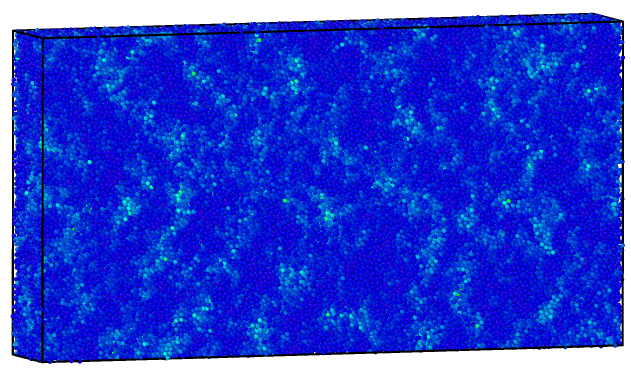
\includegraphics[width=10cm]{Cap_1/sample.png}
 \caption[Muestra utilizada en el trabajo]{Muestra Cu$_{46}$Zr$_{54}$ utilizada como base de las simulaciones de este trabajo.}
 \label{C3:fg:sample}
\end{figure}

Cada simulación diferirá de las restantes ya sea en el tipo de carga (tensión o compresión uniaxial) o en la temperatura de simulación, siendo constante la velocidad de deformación.

Se analizarán temperaturas de 10 (cercano al cero absoluto), 100, 200, 300, 400, 500, 600 y 900 K. Se incluye el caso de simulación a 900 K, sobre $T_g$, para ver si el comportamiento mecánico es significativamente diferente. Para describir las interacciones entre átomos, un potencial de método de átomo embebido (EAM) \citep{daw84} fue adoptado, que ya ha sido usado en otros estudios sobre BMGs \citep{shimizu07,cao09,cheng08,arman10,cheng11,wang12}.

En primer lugar se emplean condiciones de borde periódicas en 3D, válidas para altas velocidades de deformación \citep{bringa05}. Todas las coordenadas atómicas son escaladas a cada paso, de acuerdo con la velocidad de deformación deseada, que en este caso es de $10^9$ /s. Antes de iniciar las deformaciones mecánicas, se realiza primero una minimización de energía usando el gradiente conjugado, y luego usamos condiciones de presión cero y temperatura constante para equilibrar la muestra a la temperatura buscada T. La \tref{C3:tb:initprops} presenta los volúmenes y densidades iniciales para los diferentes casos.

%We use 3D periodic boundary conditions, suitable for high strain rates (\cite{bringa05}). All atomic coordinates are scaled every step, according to the desired strain rate, which in this case was 10$^{9}$ /s. Before starting mechanical strain simulations, we first perform energy minimization using conjugate gradient, and then use zero-pressure conditions and constant temperature to equilibrate the sample to the desired temperature T. Table 1 lists the volumes and initial sample densities for the different cases.

\begin{table}[htp]
\begin{center}
\begin{tabular}{*{3}{c}}
\hline
Temperatura [$K$] & Volumen [$nm^{3}$] & Densidad [$\frac{g}{cm^{3}}]$ \\ \hline \hline
10K & 2909.15 & 7.1705 \\ \hline
300K & 2931.93 & 7.1147 \\ \hline
600K & 2959.54 & 7.0484 \\ \hline
900K & 2992.30 & 6.9712 \\ \hline
\end{tabular}
\end{center}
\caption[Volúmenes y densidades iniciales]{Volúmenes y densidades iniciales a diferentes temperaturas simuladas.}
\label{C3:tb:initprops}
\end{table}

Luego, se analiza la presencia de bandas de corte para las condiciones de borde antes mencionadas. Por último, se investiga la respuesta frente a condiciones de borde no periódicas.

\section{Resultados}
\label{S3_3}

\subsection{Simulación de la muestra con condiciones de borde periódicas}
\label{S3_3_1}

En el texto que continúa, presentamos resultados para esfuerzos exclusivamente uniaxiales, los cuales son apropiados para la comparación con resultados de experimentos a una velocidad de deformación muy elevada, en donde las deformaciones laterales pueden despreciarse. 

La \fref{C3:fg:sStrainTen} \cambio{grafica tensión de Von Mises versus deformación a todas las temperaturas simuladas. Luego de la deformación puramente elástica existe un decremento en la tensión de Von Mises, lo que sugiere la presencia de plasticidad. En la} \fref{C3:fg:sStrain} \cambio{se provee una estimación del fin del régimen elástico para poder observar mejor este fenómeno. Además, dadas la grandes velocidades de deformación y las grandes deformaciones, se nuclea un poro en la muestra bajo tracción, como vemos en la} \fref{C3:fg:voidSeq}, lo cual produce grandes fluctuaciones de tensión luego de aproximadamente 15\% de deformación para $T=900K$, y luego de deformaciones un poco superiores para el resto de temperaturas.

%Below we present results for purely uniaxial strain, which is appropriate for the comparison with results of experiments at very high strain rates, where lateral strains can be neglected.
%Figure 1 (a) shows our results for von Mises stress versus strain at all the simulated temperatures. After the purely elastic deformation that occurs up to about 2\% strain, there is a decrease in von Mises tension, suggestive of plasticity. In addition, due to the high strain rates and large stress, there is a void nucleation in the sample under tension, as shown in Figure 2, which leads to large stress fluctuations after about 15\% strain.

\begin{figure}[htp]
\centering
\subfloat[Tracción]{
	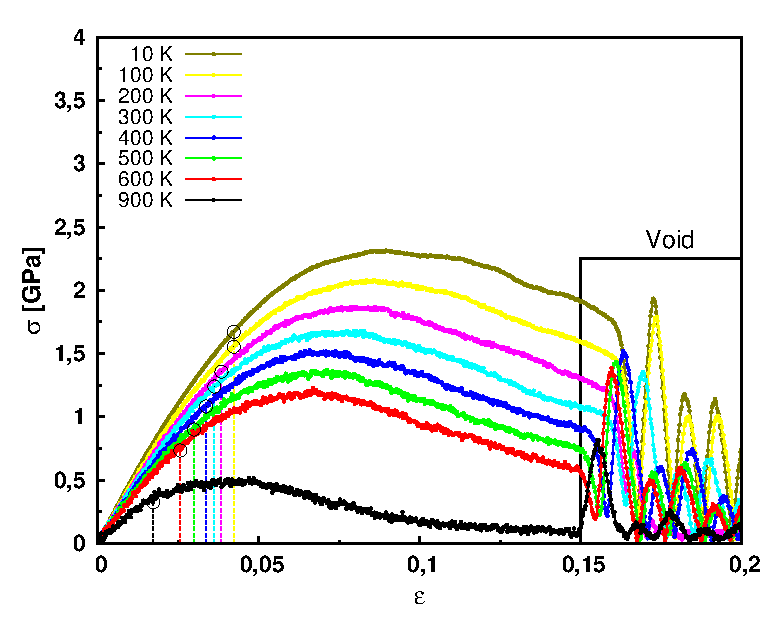
\includegraphics[width=8cm]{Cap_3/Tens_stress_strain_curve.eps}
	\label{C3:fg:sStrainTen}}
\subfloat[Compresión]{
	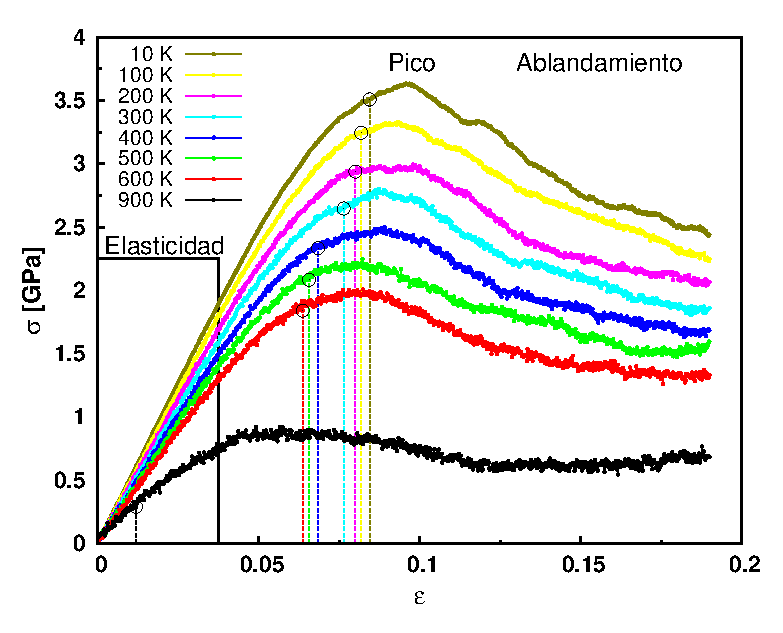
\includegraphics[width=8cm]{Cap_3/Comp_stress_strain_curve.eps}
	\label{C3:fg:sStrainComp}}
\caption[Curvas de tensión-deformación a diferentes temperaturas]{Curvas de tensión-deformación a diferentes temperaturas. Bajo tracción existen grandes fluctuaciones del esfuerzo que comienzan cuando se nuclea un poro a aproximadamente 15\% de deformación. Los círculos sobre las curvas denotan una estimación del fin de la deformación elástica, calculada como el punto donde la curva se aleja un 20\% del comportamiento elástico ideal.}
\label{C3:fg:sStrain}
\end{figure}

\begin{figure}[htp]
\centering
\begin{tabular}{C{10cm} c}
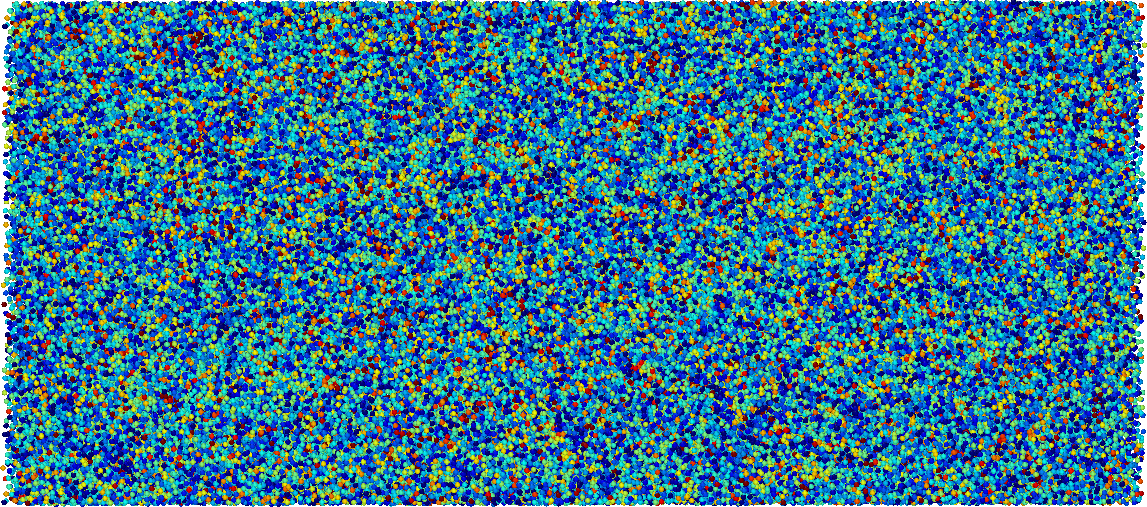
\includegraphics[width=10cm]{Cap_3/Poro_900_90000light_100-400.png} & \\
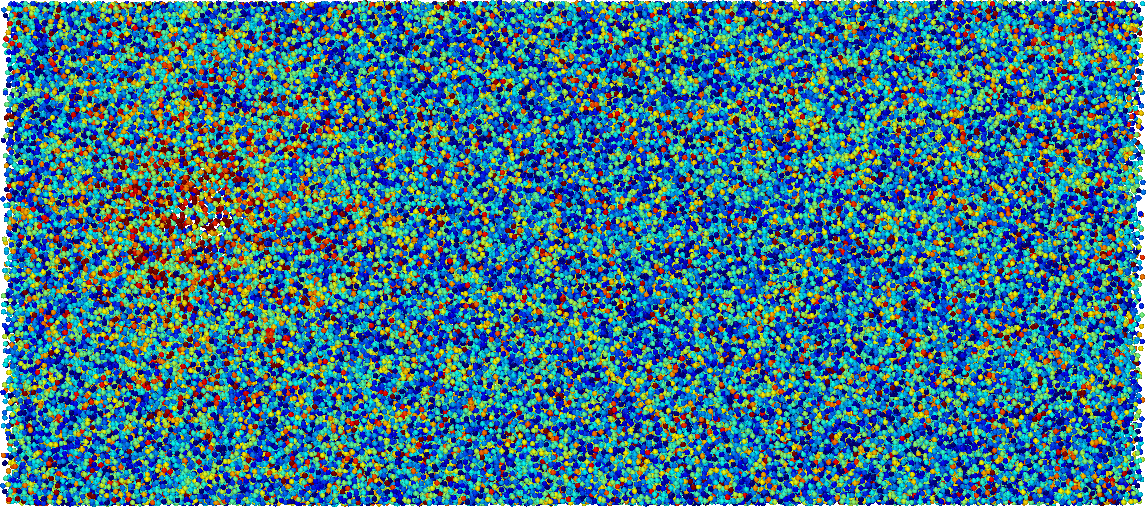
\includegraphics[width=10cm]{Cap_3/Poro_900_94000light_100-400.png} &  \multirow{3}{*}{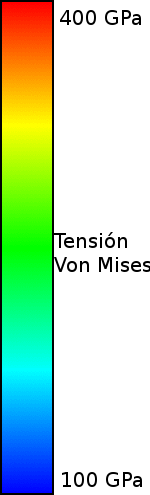
\includegraphics[width=2cm]{Cap_3/scale.png}}\\
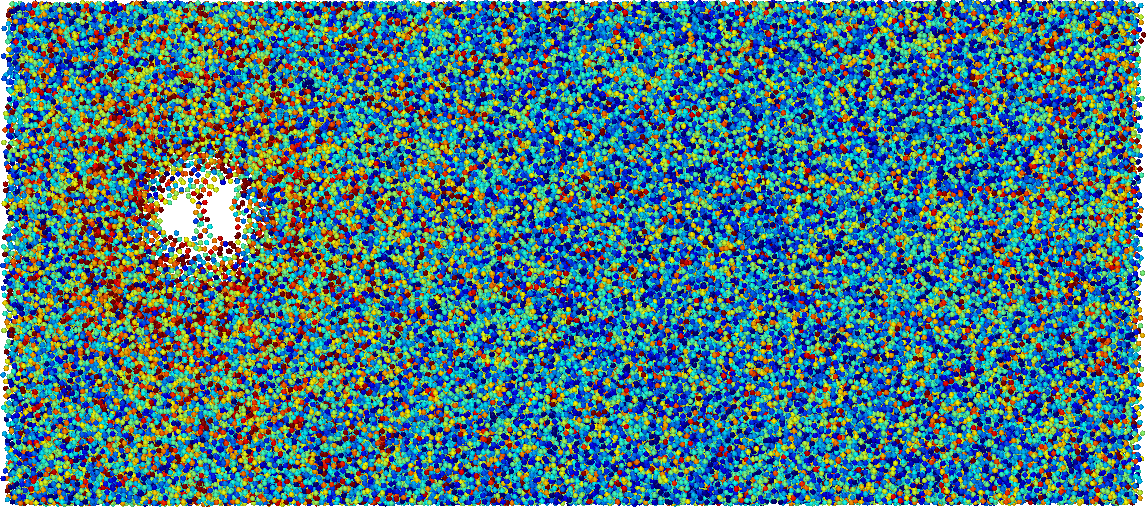
\includegraphics[width=10cm]{Cap_3/Poro_900_96000light_100-400.png} & \\
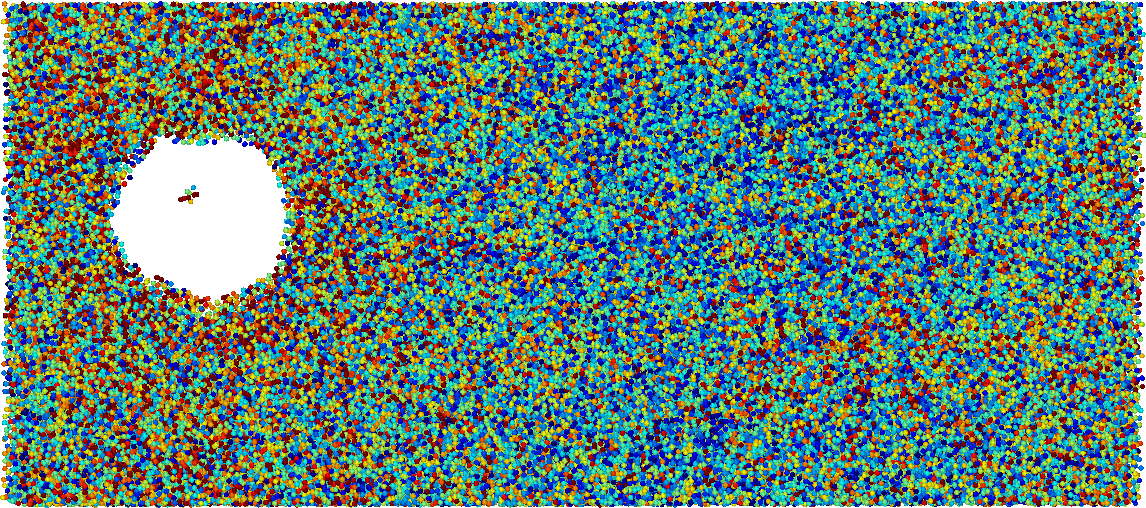
\includegraphics[width=10cm]{Cap_3/Poro_900_98000light_100-400.png} & \\
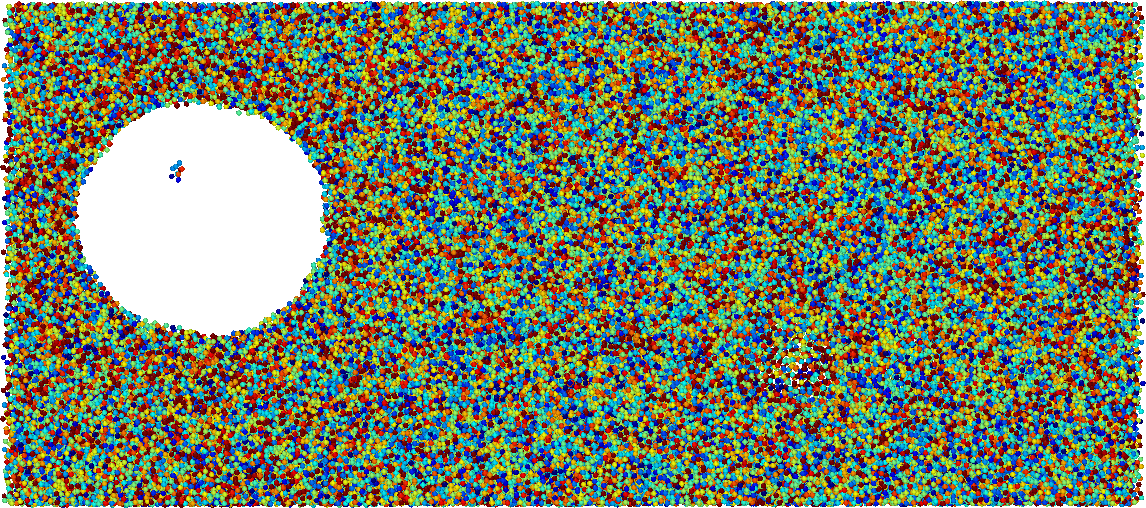
\includegraphics[width=10cm]{Cap_3/Poro_900_100000light_100-400.png} & 
\end{tabular}
\caption[Nucleación de un poro bajo tracción a 900 K.]{Nucleación de un poro bajo tracción a 900 K. Los valores de deformación son, de arriba a abajo: $\epsilon$ = 0.140, $\epsilon$ = 0.144, $\epsilon$ = 0.146, $\epsilon$ =0.148 y $\epsilon$ =0.15. Una nucleación similar es observada a temperaturas más bajas.}
\label{C3:fg:voidSeq}
\end{figure}

Calculamos las propiedades mecánicas y proponemos la siguiente forma funcional como aproximación del comportamiento térmico:

%We calculate mechanical properties, and propose the following simple functional form as an approximation for the thermal behavior:

\begin{equation}\label{C3:eq:thermalFit}
y = A_{1}\cdot \mathrm{e}^{\frac{-T}{T_{0}}}
\end{equation}

donde $A_{1}$ y $T_{0}$ son parámetros. Esta forma funcional es frecuentemente usada para fenómenos activados térmicamente. En las Tablas \ref{C3:tb:initPropsTen} y \ref{C3:tb:initPropsComp} presentamos los valores para los coeficientes de la \eref{C3:eq:thermalFit} obtenidos de las curvas mostradas en las Figuras \ref{C3:fg:youngVsT} a \ref{C3:fg:peakVMises1218VsT}. Puede verse que las regresiones son razonables. El coeficiente de correlación ($R^2$) es mayor a 0.9 en todos los casos, haciendo razonable nuestra aproximación funcional simple.
	
%where $A_{1}$ and $T_{0}$ are parameters. This functional form is often used for thermally activated phenomena. In Tables 2-3 we present the values for the coefficients of equation (1) obtained from the curves shown in Figures 3-6. It can be seen that the fits are reasonable. The correlation coefficient (R2) is greater than 0.9 in all cases, thus making our simple functional fit reasonable. Of course, further studies including many more temperature values are needed to truly test the fits. 

\begin{table}[htp]
\begin{center}
\begin{tabular}{*{4}{c}}
\hline
\textbf{Tracción} & Parámetros & Valor & $R^{2}$ \\ \hline \hline
Peak Von Mises stress & A$_{1}$ & 2.29 $\pm$ 0.04 & 0.981 \\
 & T$_{0}$ & 1068.14 $\pm$ 68.02 & \\ \hline
Von Mises stress ($\epsilon$=0.12) & A$_{1}$ & 2.21 $\pm$ 0.02 & 0.998 \\
 & T$_{0}$ & 587.05 $\pm$ 13.45 & \\ \hline
Young Modulus & A$_{1}$ & 49.42 $\pm$ 0.38 & 0.990 \\
 & T$_{0}$ & 1924.38 $\pm$ 87.18 & \\ \hline
Yield Stress & A & 0.060 $\pm$ 0.002 & 0.972 \\
 & B & -0.037 $\pm$ 0.003 & \\ \hline
\end{tabular}
\end{center}
\caption[Coeficientes de la regresión para tracción]{Coeficientes de la regresión para tracción.}
\label{C3:tb:initPropsTen}
\end{table}

\begin{table}[htp]
\begin{center}
\begin{tabular}{*{4}{c}}
\hline
\textbf{Compresión} & Parámetros & Valor & $R^{2}$ \\ \hline \hline
Peak Von Mises stress & A$_{1}$ & 3.68 $\pm$ 0.03 & 0.997 \\
 & T$_{0}$ & 1020.16 $\pm$ 25.88 & \\ \hline
Von Mises stress ($\epsilon$=0.18) & A$_{1}$ & 2.64 $\pm$ 0.08 & 0.972 \\
 & T$_{0}$ & 824.98 $\pm$ 65.21 & \\ \hline
Young Modulus & A$_{1}$ & 52.22 $\pm$ 0.53 & 0.985 \\
 & T$_{0}$ & 1757.38 $\pm$ 96.61 & \\ \hline
Yield Stress & A & 0.125 $\pm$ 0.002 & 0.985 \\
 & B & -0.068 $\pm$ 0.003 & \\ \hline
\end{tabular}
\end{center}
\caption[Coeficientes de la regresión para compresión]{Coeficientes de la regresión para compresión.}
\label{C3:tb:initPropsComp}
\end{table}

Como es de esperarse, el módulo de elasticidad, la tensión máxima de Von Mises y la tensión de fluencia, todos decrecen con el aumento de la temperatura. Obtenemos un comportamiento suave incluso cuando T supera a $T_g$, como puede verse en las Figuras \ref{C3:fg:youngVsT} a \ref{C3:fg:peakVMises1218VsT}.

%As expected, the elastic modulus, peak von Mises stress and yield stress, all decrease with increasing temperature. We obtained a smooth behavior even when T is above $T_g$, as seen in Figures 3-6.

\begin{figure}[htp]
\centering
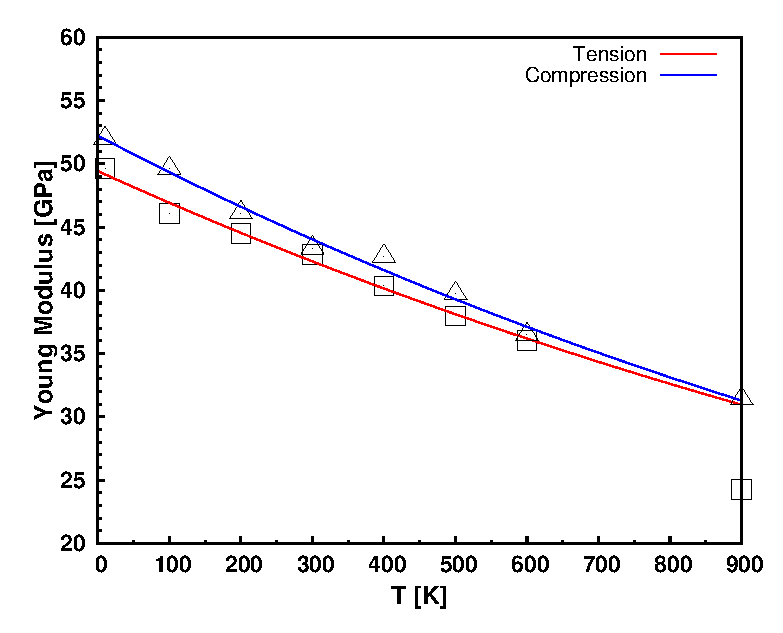
\includegraphics[width=10cm]{Cap_3/young_T_both.eps}
\caption[Aproximación módulo de Young-temperatura]{Aproximación módulo de Young-temperatura.}
\label{C3:fg:youngVsT}
\end{figure}

\begin{figure}[htp]
\centering
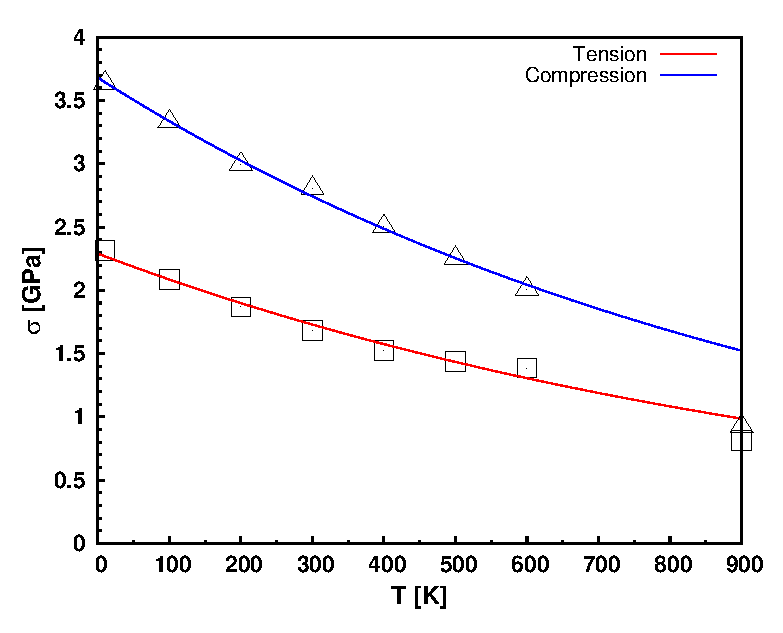
\includegraphics[width=10cm]{Cap_3/peakstress_T_BOTH.eps}
\caption[Aproximación tensión de Von Mises máxima-temperatura]{Aproximación tensión de Von Mises máxima-temperatura.}
\label{C3:fg:peakVMisesVsT}
\end{figure}

\begin{figure}[htp]
\centering
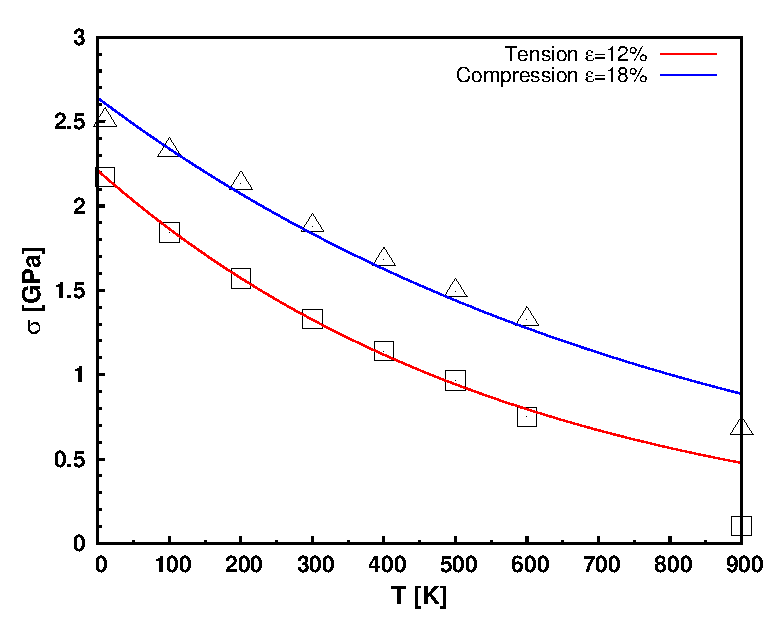
\includegraphics[width=10cm]{Cap_3/defstress_T_BOTH.eps}
\caption[Aproximación tensión de Von Mises-temperatura]{Aproximación tensión de Von Mises-temperatura. En tracción se utilizaron tensiones a deformaciones más bajas para evitar las fluctuaciones debidas a la nucleación del poro.}
\label{C3:fg:peakVMises1218VsT}
\end{figure} 

\cite{cheng11} buscó describir el comportamiento de una muestra sometida a esfuerzos cortantes puros al inicio de la plasticidad  como una función de algunas variables, incluyendo la temperatura, basándose en un CSM (modelo de corte cooperativo). Sus cálculos dieron una dependencia de la temperatura de la forma $(T/T_g)^{2/3}$. Tratamos de comparar este comportamiento con nuestros resultados. Simplificando la expresión en \cite{cheng11}, obtuvimos la siguiente expresión:

%\cite{cheng11} attempted to describe the behavior of the onset of plasticity under pure shear, as a function of several variables, including temperature, based on a CSM (cooperative shear model). The resulting temperature dependence was (T/$T_g$)2/3, and we try to apply this behavior to our results. Simplifying the expression in \cite{cheng11}, we obtain the following expression:

\begin{equation}\label{C3:eq:onsetPlast}
\frac{\sigma{}_{y}}{G} = A+B\left( \frac{T}{T_g} \right)^{2/3}
\end{equation}

donde $\sigma{}_{y}$ es la tensión de fluencia, mientras que A y B son parámetros que se deben ajustar. Para obtener la tensión de fluencia en nuestras simulaciones utilizamos la siguiente regla: asumimos que la plasticidad comienza cuando la curva esfuerzo-deformación se aleja un 20\% del comportamiento elástico, el cual lo extrapolamos a partir de puntos obtenidos a deformaciones muy bajas (menores a $\epsilon$=1\%). En las Tablas \ref{C3:tb:initPropsTen} y \ref{C3:tb:initPropsComp} presentamos valores para los coeficientes de la \eref{C3:eq:onsetPlast} obtenidos para las curvas que se muestran en la \fref{C3:fg:fitDosTercios}. En esta figura comparamos las curvas ajustadas para tracción y compresión con el resultado de \cite{johnson05}, quien obtuvo, para  deformación cortante pura, la siguiente expresión:

%where $\sigma{}_{y}$ is the yielding stress, while A and B are parameters of the fit. To obtain the yield stress in our simulations we assume that plasticity starts when the stress-strain curve departs 20\% from the linear elastic behavior extrapolated from very low strains (below $\epsilon$=1\%). In Tables 2-3 we present the values for the coefficients of equation (2) obtained for the curves shown in Figure 6. In this figure we compare the fittings for tension and compression with the result from \cite{johnson05}, who obtained, for experiments under pure shear deformation the following expression:

\begin{equation}\label{C3:eq:johnsonSamwer}
\frac{\tau _{y}}{G} = 0.036-0.016\left( \frac{T}{T_g} \right)^{0.62}
\end{equation}

donde $\tau _{y}$ es la tensión de fluencia cortante. Observamos que la \eref{C3:eq:onsetPlast} puede aproximar relativamente bien tanto la tracción como la compresión uniaxial. Hay ciertas discrepancias con la aproximación experimental de la \eref{C3:eq:johnsonSamwer}, pero notamos que los coeficientes de la aproximación tienen grandes márgenes de error, y los datos muestran mucha dispersión. Por ejemplo, el exponente es 0.62 $\pm$ 0.2.
	
%where $\tau _{y}$ is the shear yield strength .We observe that equation (2) fits both uniaxial tension and compression quite well. There are discrepancies with the experimental fit from equation (3), but we note that the coefficients in that fit had large error bars, and data showed large dispersion. For instance, the exponent was 0.62 $\pm$ 0.2.

\begin{figure}[htp]
\centering
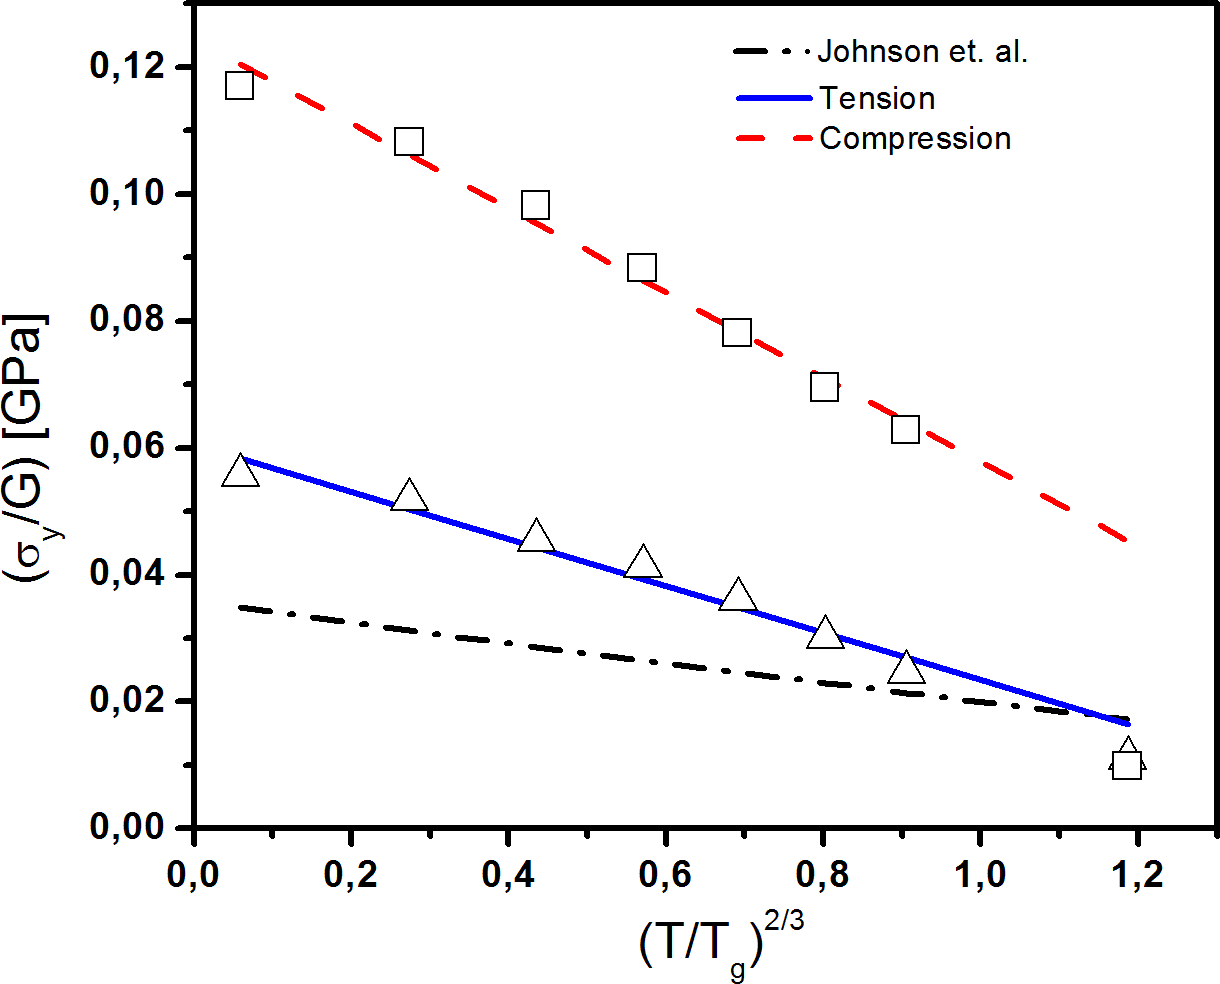
\includegraphics[width=10cm]{Cap_3/Fit2_Tercios.png}
\caption[Aproximación tensión de fluencia-temperatura]{Aproximación tensión de fluencia-temperatura. Utilizamos los valores experimentales de $T_g$ y G \citep{johnson05} para normalizar nuestros resultados.}
\label{C3:fg:fitDosTercios}
\end{figure}

La \fref{C3:fg:sampleTen} muestra la tensión de Von Mises a nivel atómico para la muestra completa (tracción a $T=300K$). A pesar de la evidencia de comportamiento plástico en las curvas esfuerzo-deformación, no observamos evidencia de bandas de corte.

%Figure 7 shows atomic von Mises stress for the complete sample in the case of tension at T=300K. Despite the evidence of plastic behavior in stress-strain curves, we do not observe evidence of shear bands.

De acuerdo a un estudio en nanocables de vidrio metálico \citep{xiao12}, la presencia de bandas de corte depende fuertemente de la velocidad de enfriamiento del vidrio. En este caso, para las velocidades de enfriamiento utilizadas en la creación de nuestra muestra, podría suceder que no se observen bandas de corte. Sin embargo, más adelante en esta sección se observarán posibles bandas de corte incipientes al graficar la deformación atómica en lugar de la tensión de Von Mises.

%According to a recent study in metallic glass nanowires (\cite{xiao12}), the presence of shear bands strongly depends on the quenching rate of the glass. In this case, for the quenching rates used in the creation of our sample, shear bands should not be observed, as shown in Figure 7.

\begin{figure}[htp]
\centering
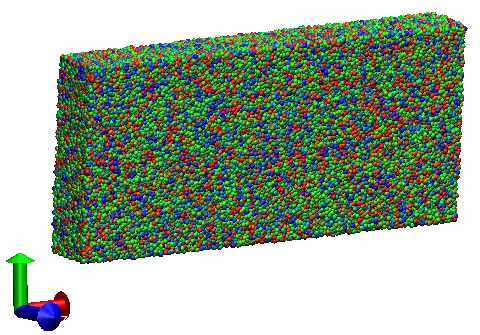
\includegraphics[width=10cm]{Cap_3/All_300K_6pstrain_sacale100-280_Trac.png}
\caption[Vista de la muestra a $\epsilon$=6\%, bajo tracción uniaxial, a T=300 K]{Vista de la muestra a $\epsilon$=6\%, bajo tracción uniaxial, a T=300 K. Los colores representan la tensión de Fon Mises. No se observan SB. La visualización fue realizada con VMD \citep{humphrey96}. Resultados similares se observan a otras temperaturas simuladas.}
\label{C3:fg:sampleTen}
\end{figure}

Cuando deformamos el vidrio metálico mediante compresión uniaxial podemos observar un comportamiento similar de las curvas esfuerzo-deformación mostradas en la \fref{C3:fg:sStrainComp} con respecto a las curvas de tracción mostradas en la \fref{C3:fg:sStrainTen}, siempre a deformaciones menores al 15\%. Luego del 15\% deformación las curvas de compresión tienen una forma suave debido a que no hay nucleación de poros.

%When the metallic glass deforms under uniaxial compression we can observe a similar behavior in the stress-strain curves shown in Figure 1 (b) to the curves corresponding to tension in Figure 1 (a), for strains below 15\%. However, since there is no void nucleation above 15\%, the behavior of the curves is smooth even at very high strains.

Las Figuras \ref{C3:fg:youngVsT} a \ref{C3:fg:fitDosTercios} muestran las mismas aproximaciones que las usadas para tracción. Las aproximaciones también son razonables, incluso con una ecuación de aproximación simple como la mostrada en la \eref{C3:eq:thermalFit}.

%Figures 3-6 show the same type of fit that the one used for tension, and there is also a reasonable adjustment, even with the simple functional form shown in equation (1).

La \fref{C3:fg:sampleComp} muestra que, de igual manera que en la muestra bajo tracción, no se observan bandas de corte.

%Figure 8 shows that, similarly to the sample under tension, no shear bands are observed, as expected given the high quenching rate of the glass used here.

\begin{figure}[htp]
\centering
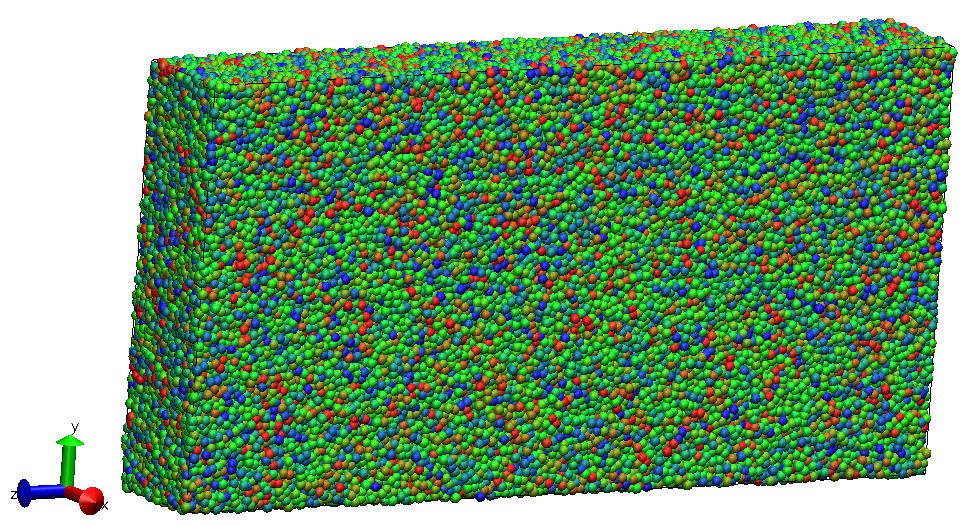
\includegraphics[width=10cm]{Cap_3/All_300K_6pstrain_sacale100-400_Comp.png}
\caption[Vista de la muestra a $\epsilon$=6\%, bajo compresión uniaxial, a T=300 K]{Vista de la muestra a $\epsilon$=6\%, bajo compresión uniaxial, a T=300 K. Los colores representan la tensión de Von Mises. No se observan SB. La visualización fue realizada con VMD \citep{humphrey96}. Resultados similares se observan a otras temperaturas simuladas.}
\label{C3:fg:sampleComp}
\end{figure}

Respecto a las bandas de corte, como se mencionó previamente, es posible observarlas graficando la deformación atómica en vez de la tensión de Von Mises. Para esto se utiliza la herramienta Ovito, la cual utiliza el procedimiento descripto en \cite{shimizu07} para calcular la deformación atómica. La \fref{C3:fg:SBs} muestra el resultado.

\begin{figure}[htp]
\centering
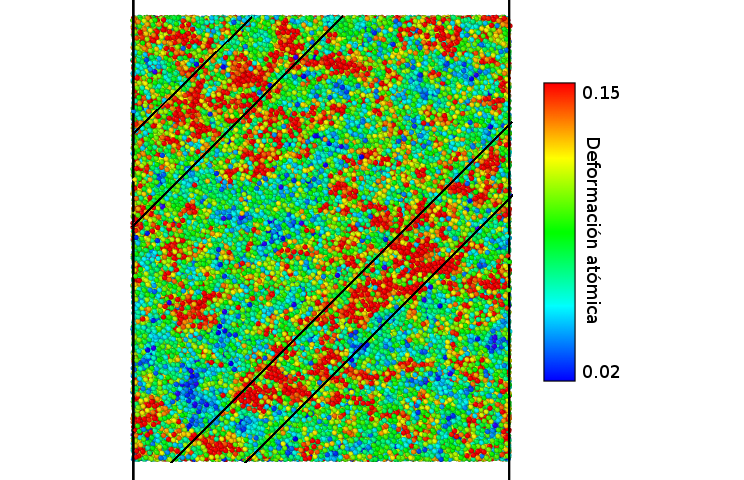
\includegraphics[width=10cm]{Cap_3/ShearBand.png}
\caption[Corte de la muestra a $\epsilon$=14\%, bajo compresión uniaxial, a T=300 K.]{Corte de la muestra a $\epsilon$=14\%, bajo compresión uniaxial, a T=300 K. La visualización fue realizada con Ovito \citep{stukowski10}. Se eliminan los efectos de la deformación homogénea para poder apreciar mejor la deformación heterogénea producto de las bandas de corte.}
\label{C3:fg:SBs}
\end{figure}

Es posible apreciar que hay bandas de corte incipientes que se forman con una dirección predominantemente diagonal, a prácticamente $45º$ con respecto a la dirección de aplicación de la fuerza. Las bandas de corte representan deformación heterogénea, lo cual puede llevar a la falla frágil del material. Esto es algo importante a tener en cuenta ya que puede reducir considerablemente la vida útil del material. En capítulos subsiguientes trataremos algunos métodos para retardar la propagación de bandas de corte.

\subsection{Simulación de la muestra con condiciones de frontera libres.}
\label{S3_3_2}

\cambioGrande{ESTA SECCION ENTERA}

Para investigar la influencia de las condiciones de borde, se realizaron simulaciones con condiciones de frontera laterales libres. Estas simulaciones son similares a aquellas realizadas sobre nanocables de vidrio metálico en \cite{xiao12}. Las Figuras \ref{C3:fg:libresTen}, \ref{C3:fg:cross} y \ref{C3:fg:libresComp} muestran los resultados obtenidos. Se ha graficado la deformación atómica y no la tensión de Von Mises, ya que esta última no provee resultados relevantes, al igual que en la Sección anterior.

Bajo tracción, \fref{C3:fg:libresTen}, hay una pequeña disminución de la sección transversal de la muestra, como era de esperar. Esto puede ser observado con mayor detalle en la \fref{C3:fg:cross}. También podemos observar que la forma de la sección transversal cambia de rectangular a elíptica, debido a un efecto de minimización de la energía de superficie. Bajo compresión, \fref{C3:fg:libresComp}, se observa pandeo.

%To verify that the absence of shear bands is not due to periodic conditions during deformation, simulations were carried out with free lateral boundary conditions, as shown in Figure 10. Under tension there is a slight decrease in the cross section of the sample, as expected. This is shown in Figure 11. We can also observe that the shape of the cross section has changed from rectangular to elliptical, due to surface energy minimization.

\begin{figure}[htp]
\centering
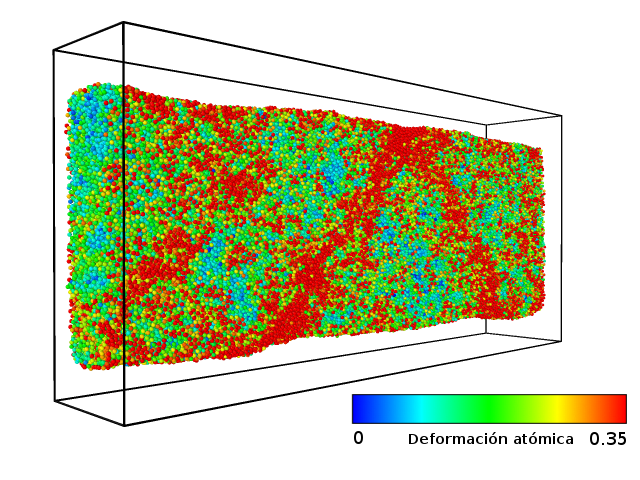
\includegraphics[width=12cm]{Cap_3/Pseudo_Free_Boundaries_ShearStrain_0_035_300K_20strain.png}
\caption[Simulación a tracción usando condiciones de frontera libres]{Simulación a tracción usando condiciones de frontera libres. $\epsilon$=0.20, T=300K.}
\label{C3:fg:libresTen}
\end{figure}

\begin{figure}[htp]
\centering
\subfloat[Sección próxima al extremo, $\epsilon$=0.]{
	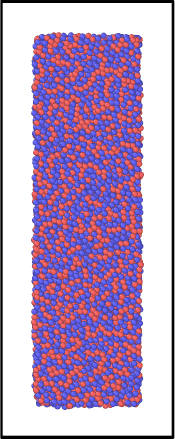
\includegraphics[width=3cm]{Cap_3/Pseudo_Free_Boundaries_0strain_transversal.png}
	\label{C3:fg:crossExtreme0}}
\subfloat[Sección próxima al extremo, $\epsilon$=0.20.]{
	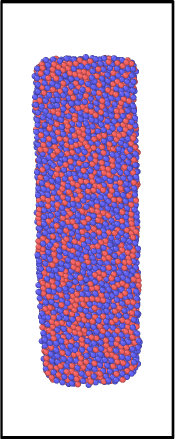
\includegraphics[width=3cm]{Cap_3/Pseudo_Free_Boundaries_20strain_transversal_esquina.png}
	\label{C3:fg:crossExtreme020}}
\subfloat[Sección central de la muestra, $\epsilon$=0.20.]{
	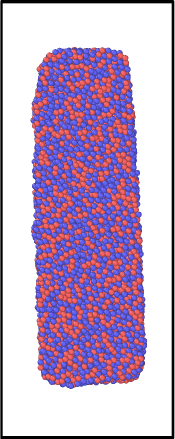
\includegraphics[width=3cm]{Cap_3/Pseudo_Free_Boundaries_20strain_transversal_centro.png}
	\label{C3:fg:crossMiddle020}}
\caption[Cortes a diferentes distancias sobre el eje z, condiciones de frontera libres]{Sección transversal a diferentes distancias sobre el eje z, para la simulación presentada en la \fref{C3:fg:libresTen}. No se aprecia estricción, incluso a altas deformaciones.}
\label{C3:fg:cross}
\end{figure}

\begin{figure}[htp]
\centering
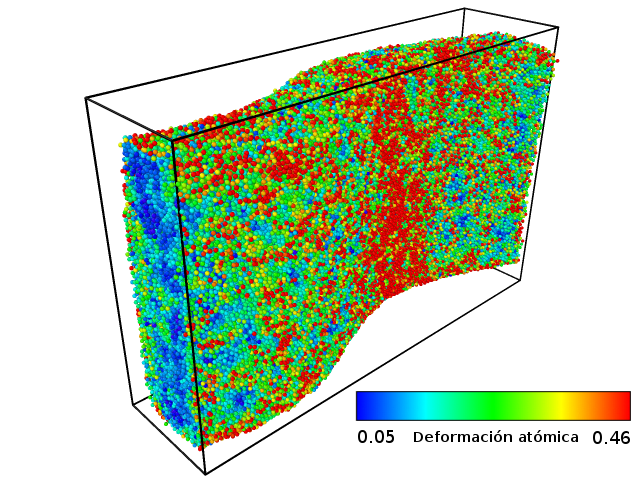
\includegraphics[width=12cm]{Cap_3/Pseudo_Free_Boundaries_ShearStrain_005_046_300K_15strain.png}
\caption[Simulación a compresión usando condiciones de frontera libres]{Simulación a compresión usando condiciones de frontera libres. $\epsilon$=0.15, T=300K.}
\label{C3:fg:libresComp}
\end{figure}

En el caso de tracción la formación de bandas de corte es más evidente que en la simulación con condiciones de frontera periódicas (\fref{C3:fg:SBs}). Existen dos bandas de corte principales, las cuales se orientan a $45º$ con respecto a la dirección de aplicación de la fuerza. También se observa que las SB se encuentran en un punto en común, lo cual hace pensar que algún defecto de superficie puede haber sido el catalizador de la deformación heterogénea. En el caso de compresión la máxima deformación se da en las zonas de mayor curvatura debido al pandeo de la muestra. La deformación es superior en el lado que se encuentra comprimido, como bien puede observarse en la \fref{C3:fg:libresComp}.

%These simulations are similar to those of metallic glass nanowires seen in \cite{xiao12}. Under compression, buckling is observed. In both cases there is a lack of shear bands, as expected with the cooling rates used in our samples.



%\section{Conclusiones}


%Atomistic simulations of bulk metallic glasses (BMGs) mechanical behavior under tension and compression were performed using molecular dynamics (MD) simulations. The increase of sample temperature produces a considerable decrease of the samples elastic modulus. The same applies to maximum von Mises stress. It is observed that the elastic modules are practically the same under tension or compression at different temperatures, but the maximum stress in compression is much higher. The behavior with temperature can be adjusted reasonably well with an exponential decay with temperature, typical of thermal activated phenomena.

%No shear bands are observed, which is to be expected given that our glass was generated with very high quenching rates. Since no shear bands are observed in our simulations, the identification of plasticity is complex. Surely there are shear areas, "shear transformation zones" (STZ), composed of a few atoms that experience high shear stresses. The identification of these areas requires a very detailed observation of the sample, involving much longer simulations than those used here. An alternative to study plasticity is the examination of Voronoi polyhedra, which can help to identify these areas. Such studies are in progress.

%In the future, using more powerful computational resources than available for this work, we plan to create samples with quenching rates orders of magnitude slower, with the aim to observe the possible formation of shear bands.

%A detailed understanding of the influence of temperature, quenching rates, etc., in the mechanical properties of metallic glasses will allow obtaining necessary properties for their application in new technologies, including applications under extreme conditions, such as aerospace missions or materials in nuclear reactors. Studies like the one presented here will contribute to this understanding and accelerate novel material development. 